%!TEX root = ../dokumentation.tex

\chapter{Umsetzung}

Im folgenden wird nun detailliert auf das entwickelte Konzept eingegangen und deren Funktionsweisen erläutert.

%title wird unter dem Bsp. abgedruckt
%caption wird im Verzeichnis abgedruckt
%label wird zum referenzieren benutzt, muss einzigartig sein.

\section{Voraussetzungen}
Für die Nutzung des Audioplayer auf dem Raspberry Pi bzw. für die weitere Entwicklung, müssen vorerst einige Anpassungen und Installationen getätigt werden. Diese Schritte sind notwendig damit der Audioplayer wie vorgesehen funktioniert und keine unvorhergesehen Zustände entstehen.

\subsection{Pakete installieren und Raspberry Pi updaten}
Standardmäßig besitzt der Raspberry Pi das Betriebssystem \textit{Raspbian}. Dieses gilt es zuerst auf die neuste Version zu aktualisieren. Zusätzlich werden alle installierten Pakete des System auf die neuste Version zu aktualisieren. Dieses Vorhaben wird mit den folgenden Befehlen durchgeführt:
\begin{lstlisting}
sudo apt-get update 
sudo apt-get upgrade 
sudo apt-get install rpi-update 
sudo rpi-update
\end{lstlisting}
Die ersten drei Befehle werden mit \ac{APT} ausgeführt. \ac{APT} ist ein Paketverwaltungssystem welches für den Bereich der Debian Betriebssysteme entwickelt wurde. Das Tool verwaltet die gesamten Debian Pakete und somit auch die installierten Applikationen auf dem Raspberry Pi \autocite{apt-debian-wiki_2019}. Sudo wird hier überall gebraucht, da für alle Aktionen sudo Rechte benötigt werden.
Mit dem Befehl \textit{sudo apt-get update} werden alle Paketquellen neu eingelesen - also ein großes Lexikon wo man was in welcher Version finden kann.
Mit dem Befehl \textit{sudo apt-get upgrade} werden alle bereits installierten Paket auf die in den Paketquellen vorhandene neuste Version aktualisiert. Dabei werden keine neuen Pakete installiert oder alte nicht mehr benötigte Abhängigkeiten entfernt. \autocite{apt-get-wiki_2019}
Mit dem Befehl \textit{apt-get install rpi-update} wird das Paket \textit{rpi-update} mit allen seinen Abhängigkeiten heruntergeladen und installiert. Das Paket ist ein automatisiertes Skript zum updaten des Raspberry Pi's Betriebssystem auf die neuste Version.
Als letzten Schritt wird nun das Paket \textit{rpi-update} ausgeführt und der Raspberry Pi lädt automatisch das neuste passende Betriebssystem herunter und installiert es. Dabei gehen keine Daten verloren.
\\
Nachdem der Raspberry Pi sich erfolgreich aktualisiert hat, müssen nun noch die jedenfalls benötigten Pakete installiert werden. Dies wird mit den folgenden Befehlen gemacht.
\begin{lstlisting}
sudo apt-get install portaudio19-dev
sudo apt-get install libmpg123-dev
sudo apt-get install mp3info 
\end{lstlisting}

\subsection{Anpassungen für Entwicklungszwecke}
hier bla bla

\subsection{Nötige Schritte für die Nutzung}
hier auch bla bla

\section{Konzept}
Hier kommt der Scheiß ist zustand rein
\begin{figure}[h]
	\centering
	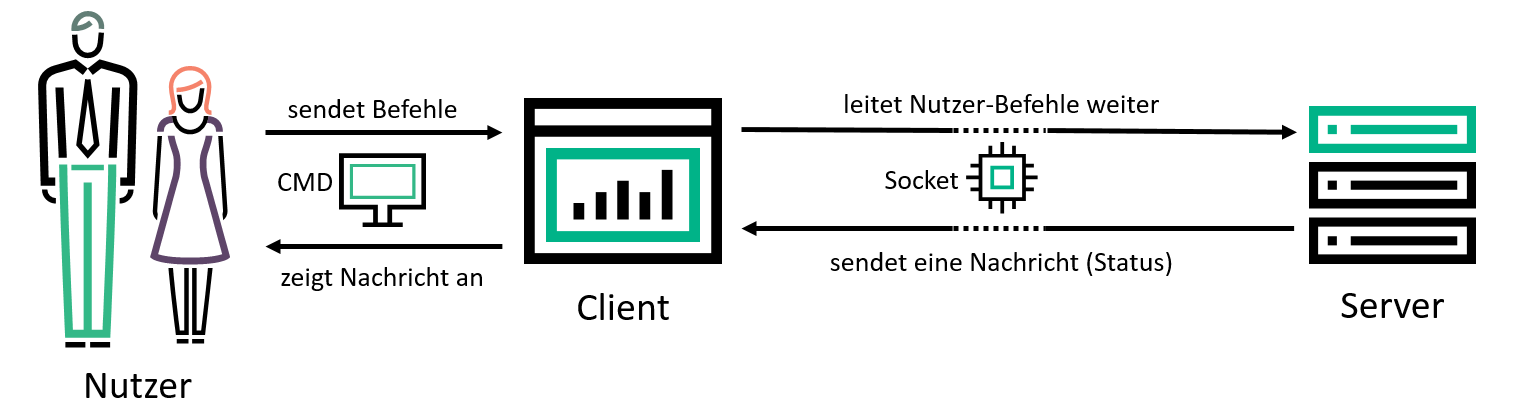
\includegraphics[scale=0.5]{Audioplayer_Konzept.png}
	\caption{Audioplayer - Konzept}
	\label{img:grafik-RaspberryPi3}
\end{figure}
\newline

\subsection{Konzept des Clients}
Hier kommt der Scheiß ist zustand rein

1. Holt sich die Config(da stehen alle Sachen drinnen wie Ort des Sockets und blabla)\\
2. Setzt den Logger auf \\
3. Überprüft ob der Server bereits läuft, wenn nicht dann startet er den Server und wartet solange bis er hochgefahren ist und die Verbindung zum socket besteht. \\
4. Überprüft ob Übergabeparameter(Kommando) übergeben wurden. Wenn nicht dann Programm beenden, wenn doch dann Parsen den Übergabewerte \\
5. Packen der geparsten Informationen in ein JSON Format und senden dies JSON über den Socket an den Server. \\
6. Beenden des Clients \\

\subsection{Konzept des Servers}

1. Holt sich die Config(da stehen alle Sachen drinnen wie Ort des Sockets und blabla)\\
2. Setzt den Logger auf \\
3. Setzt den Socket auf \\
4. Starten Pulseaudio \\
5. Hört den Socket ab \\
	5.1 Falls nichts kommt...warten \\
	5.2 Falls was reinkommt - JSON Parsen und das gewünschte Kommando ausführen.\\
	

\section{Kommunikation über Sockets}
Sockets erklären und kurz erläutern warum wir die verwendet haben.\\
\\
Ein Socket (von engl. Sockel, Steckverbindung oder Steckdose) ist ein vom Betriebssystem bereitgestelltes Objekt, das als Kommunikationsendpunkt dient. Ein Programm verwendet Sockets, um Daten mit anderen Programmen auszutauschen. Das andere Programm kann sich dabei auf demselben Computer (Interprozesskommunikation) oder einem anderen, via Netzwerk erreichbaren Computer befinden. Die Kommunikation über Sockets erfolgt in der Regel bidirektional, das heißt, über das Socket können Daten sowohl empfangen als auch gesendet werden.

\section{Funktionen des Programms}
Hier kommen die Scheiß Funktionen rein, alle Beschreiben und vll. kurz erläutern evtl. an einer Zeichnung wie diese Ablaufen.

\href{https://github.com/alexanderklapdor/RaspberryPi_Go_Audioplayer#commands-of-the-client}{Kommandos}
\\
\href{https://github.com/alexanderklapdor/RaspberryPi_Go_Audioplayer#console-arguments}{Console-Arguments}


\section{Bedienung des Programms}
Beispiele für die Bedienung reinmachen ( Ordner abspielen, Loop, Playlist, blabla)

